\documentclass[11pt]{article}
\usepackage[a4paper,margin=2.5cm]{geometry}
\usepackage[T1]{fontenc}
\usepackage[utf8]{inputenc}
\usepackage{amsmath,amssymb,amsthm}
\usepackage{booktabs,array}
\usepackage{graphicx}
\usepackage{xcolor}
\usepackage[numbers,sort&compress]{natbib}
\usepackage[colorlinks=true,linkcolor=blue!50!black,citecolor=blue!50!black,urlcolor=blue!50!black]{hyperref}
\graphicspath{{../../examples/}}

\newtheorem{proposition}{Proposition}
\newtheorem{remark}{Remark}
\newcommand{\qgZ}{qg_Z}
\newcommand{\qgX}{qg_X}
\newcommand{\mqg}{\overline{qg}_Z}
\newcommand{\Tr}{\operatorname{Tr}}
\newcommand{\fb}{\texttt{fake\_brisbane}}

\title{The register-mean polar bias as a symmetry witness:\\
error mitigation, constrained optimization and qubit characterization in qg units}
\author{Vicente Humberto Monteverde\\
\small Universidad del Museo Social Argentino (UMSA), Argentina\\
\small ORCID 0000-0001-8884-4811}
\date{\small Draft of 26 September 2026}

\begin{document}
\maketitle

\begin{abstract}
In the qg framework~\cite{monteverde2026qang} a qubit is described by its polar bias
$\qgZ=\langle\sigma_z\rangle$. When a circuit conserves a Hamming weight, the average of $\qgZ$
over the register is fixed in advance: $\mqg=1-2N/n$ for $N$ excitations on $n$ qubits. This one
number is a reference-free witness of noise that changes the conserved quantity, and its shot-level
version is the known symmetry-verification filter~\cite{bonetmonroig2018,mcardle2019}. We measure
when the witness and the filter help, and when they do not, on six problems with classical controls,
using calibration-based and vendor noise models. (i) On H$_2$ the filter lowers the energy error from
18 to 5.5~mHa, below Hartree--Fock (20.3~mHa), and it stays below Hartree--Fock along the
dissociation curve. (ii) Across noise channels the witness predicts the outcome: it moves under T1
and the filter removes 94--95\% of the error for free, while under dephasing it stays at its ideal
value and the filter does nothing. Zero-noise extrapolation is complementary and fails on idle
decoherence; the combination reaches $2.0\pm3.9$~mHa. (iii) With separate spin-up and spin-down
witnesses, a second filter pays off only when a spin-leak witness is nonzero. Qubit routing on a
heavy-hex device creates such leak in 1D Hubbard dynamics. (iv) In QAOA with an ``exactly $K$''
constraint, the filter doubles the success probability of the constraint-preserving ansatz. Penalty
QAOA at depth $\le2$ does not beat a random feasible guess, and a greedy algorithm beats all quantum
variants. (v) The witness relies on calibrated readout. A heralded sweep separates thermal
population from asymmetric readout error, which the standard calibration conflates, and gives an
unbiased effective temperature ($\pm1$~mK) together with $T_1$ and $T_2$. We also report where the
method stops: a 6-qubit LiH circuit and Hubbard circuits beyond $\sim$190 two-qubit gates, where
the witness correctly reports unital scrambling. No result is a quantum advantage over classical
computation. Every number is reproduced by a script and pinned by a regression test.
\end{abstract}

\section{Introduction}

Near-term quantum computations are limited by noise, and error mitigation trades extra
measurements or post-processing for lower bias~\cite{temme2017,li2017,kandala2019}. When the target
state has a known symmetry, such as particle number in a fermionic simulation or a cardinality
constraint in optimization, outcomes that break it can be discarded. This is symmetry
verification~\cite{bonetmonroig2018,mcardle2019}.

This paper reads that symmetry in the language of the qg framework~\cite{monteverde2026qang}, where a
qubit is described by $\qgZ=\cos\theta=\langle\sigma_z\rangle$. The contribution is not the filter,
which is known, but three things around it:
\begin{enumerate}
\item a single, reference-free number, the register mean $\mqg$, that tells \emph{before} any
mitigation whether noise is breaking the symmetry and in which direction;
\item a systematic comparison, with classical baselines and a standard mitigation method (zero-noise
extrapolation), of when the filter helps and when it cannot;
\item a calibration protocol for the readout on which the witness depends, written in the same
units.
\end{enumerate}
We state limits alongside results. In particular, every problem studied is classically easy at the
sizes used, so the comparisons rank strategies for a quantum computation and do not claim a
quantum advantage.

\section{The witness}\label{sec:witness}

\begin{proposition}\label{prop:witness}
Let $W=\sum_i(1-Z_i)/2$ count the qubits in $|1\rangle$. For any state supported on the eigenspace
$W=N$,
\begin{equation}
\mqg\equiv\frac1n\sum_{i=1}^n\Tr(\rho\,Z_i)=1-\frac{2N}{n}.
\end{equation}
\end{proposition}
\begin{proof}
$\frac1n\sum_iZ_i=1-\frac2nW$, and $W=N$ on the support of $\rho$.
\end{proof}

In the Jordan--Wigner encoding $W$ is the electron number. In a ``choose exactly $K$'' problem it
is the cardinality. For a circuit that conserves $W$, the ideal $\mqg$ is therefore known for every
value of the parameters. We use four quantities, all read from the same Z-basis shots:
\begin{itemize}
\item the \emph{witness} $\mqg$. Amplitude damping (T1) moves it towards $+1$. Unital noise
(depolarizing, dephasing) moves it towards the value of a maximally mixed register, 0;
\item the \emph{kept fraction}, i.e.\ the probability of the shots with $W=N$. It is 1 ideally and
$\binom{n}{N}/2^n$ for a maximally mixed register, which marks the noise floor;
\item the \emph{filter}: keep only those shots and renormalize (symmetry verification);
\item for two conserved numbers (spin up and spin down), one witness per register and a
\emph{spin leak}, the fraction of right-$N$ shots in the wrong spin sector.
\end{itemize}
Observables measured in rotated bases, such as the $XXYY$ terms of a molecular Hamiltonian, cannot be
filtered this way. The witness is linear in $\rho$, so its estimator from counts is an unbiased
sample mean.

\paragraph{Readout.} Readout errors enter as an affine map. If a qubit reads 1 when in $|0\rangle$
with probability $e_{01}$ and 0 when in $|1\rangle$ with probability $e_{10}$, then
\begin{equation}\label{eq:affine}
\qgZ^{\rm meas}=a+b\,\qgZ,\qquad a=e_{10}-e_{01},\quad b=1-e_{01}-e_{10}.
\end{equation}
An asymmetric readout ($a\neq0$) therefore shifts the witness the way T1 does. Section~\ref{sec:char}
shows how to calibrate $a$ and $b$ without confusing them with the thermal population of the qubit.

\section{Methods}\label{sec:methods}

\paragraph{Noise models.} (a) \fb: Qiskit Aer~\cite{javadiabhari2024qiskit} with the noise model built
from an IBM device's calibration data (ECR gates, heavy-hex connectivity, thermal relaxation during
scheduled idle times, readout errors), on a chain of the best-calibrated qubits. An optional idle
delay before readout amplifies T1. (b) Controlled channels applied to every CX (so that gate
folding scales them exactly): amplitude damping, phase damping or two-qubit depolarizing noise of
strength $p$, or symmetric readout error only. (c) A generic all-to-all device dominated by
depolarizing two-qubit error (0.6\% per CX, 0.1\% dephasing, 0.5\% readout), with trapped-ion-like
figures but not a vendor calibration. (d) IonQ's \texttt{aria-1} and \texttt{forte-1} noise models,
run on IonQ's cloud simulator.

\paragraph{Mitigation.} All quantum estimates include tensored readout-error mitigation unless
stated. Zero-noise extrapolation (ZNE)~\cite{temme2017,li2017} folds every two-qubit gate $G$ into
$G^3$ and $G^5$ and extrapolates to zero noise with Richardson weights $(15,-10,3)/8$. ``ZNE + qg''
filters at every noise scale and then extrapolates.

\paragraph{Statistics.} Unless stated, 20{,}000 shots per circuit and mean $\pm$ standard deviation
over 10 simulator seeds. The references are exact classical results (FCI, exact diagonalization,
brute force) at these sizes.

\section{Chemistry}\label{sec:chem}

H$_2$ (STO-3G, 0.735~\AA) in the Jordan--Wigner encoding uses 4 qubits and 2 electrons, so the
ideal $\mqg$ is 0. A number-conserving ansatz with one parameter reaches the FCI energy without
noise. On \fb\ (Table~\ref{tab:h2}) the witness rises with the idle delay, in step with the
fraction of shots that lost an electron. The filter lowers the error $3.2\times$ below readout
mitigation alone and $3.7\times$ below classical Hartree--Fock. Its gain grows with T1. Along the
dissociation curve Hartree--Fock fails increasingly, while the filtered quantum estimate stays
within 6--20~mHa, $11\times$ below Hartree--Fock at 2.5~\AA.

\begin{table}[t]
\centering\small
\caption{H$_2$ on \fb, energy error vs FCI (mHa), mean of 3 seeds. Hartree--Fock: 20.3~mHa.}
\label{tab:h2}
\begin{tabular}{lcccccc}
\toprule
idle delay & $\mqg$ & kept & raw & + readout & + readout + qg filter \\
\midrule
0~$\mu$s & $+0.011$ & 0.91 & 74 & 18 & \textbf{5.5}\\
20~$\mu$s & $+0.057$ & 0.83 & 140 & 90 & \textbf{20}\\
50~$\mu$s & $+0.122$ & 0.72 & 231 & 188 & \textbf{30}\\
\bottomrule
\end{tabular}
\end{table}

\paragraph{Trapped-ion noise.} On IonQ's \texttt{aria-1} and \texttt{forte-1} noise models (2000
shots, 3 runs) the witness barely moves ($+0.004$, $+0.005$) and only 2--3\% of the shots violate
the electron number. Dropping them still lowers the error from $\sim$30 to $\sim$12~mHa, because
number-violating outcomes sit at very high energy. The run-to-run spread is about $\pm8$~mHa.

\paragraph{Spin-resolved witnesses.} H$_2$ also conserves $N_\uparrow$ and $N_\downarrow$
separately. Keeping one up and one down electron removes two more bit strings. Under depolarizing
noise on the CXs the spin leak is 1.5--5\%, and the second filter removes a further 34--37\% of the
error (23.2 $\to$ 14.7~mHa at $p=0.03$). On \fb\ the leak is below 1\% and the gain is within the
seed spread (6.5 $\to$ 5.9~mHa). The residual $\sim$5~mHa of Table~\ref{tab:h2} is in the $XXYY$
terms and in errors that preserve both numbers, not in spin leak.

\paragraph{Where it stops.} For LiH at 3.0~\AA\ (6 qubits, ideal $\mqg=1/3$) the ansatz needs 60 ECR
gates. Every quantum estimate is then $\sim9\times$ worse than Hartree--Fock, and the filter does not
help. The witness explains why: $\mqg$ falls from $+0.333$ to $+0.18$, towards 0 and not towards
$+1$. The dominant error is unital scrambling, which leaves the kept shots scrambled too.

\section{Which noise does the filter fix?}\label{sec:zne}

Table~\ref{tab:zne} compares the filter with ZNE on the same H$_2$ state. Three regularities appear
(Fig.~\ref{fig:zne}).
\begin{itemize}
\item \textbf{The witness predicts whether the filter works.} Dephasing preserves the electron
number. The witness stays at 0, every shot is kept, and the filter changes nothing; only ZNE helps.
T1 moves $\mqg$ up by about $p$, and the filter removes 94--95\% of the error with no extra circuits
and less spread than ZNE.
\item \textbf{The methods are complementary.} ZNE overshoots under T1, by $-4$ to $-6$~mHa, because
amplitude damping is not linear in the fold count, and it doubles or triples the spread. Under strong
depolarizing noise only the combination comes within a few mHa.
\item \textbf{Idle decoherence defeats ZNE.} Gate folding does not scale a 50~$\mu$s idle period
(189 $\to$ 177~mHa). The witness flags it ($+0.122$), and the filter removes 84\% of the error.
\end{itemize}
This gives a decision rule. If $\mqg$ leaves $1-2N/n$ or the kept fraction drops, apply the filter,
which is free. If the error stays large with the kept fraction near 1, the remaining noise
preserves the symmetry and needs ZNE.

\begin{table}[t]
\centering\footnotesize\setlength{\tabcolsep}{4pt}
\caption{H$_2$, error vs FCI (mHa), mean $\pm$ std over 10 seeds. Controlled noise acts on every CX.}
\label{tab:zne}
\begin{tabular}{lcccccc}
\toprule
noise & $\mqg$ & kept & readout-mitigated & + qg filter & + ZNE & + ZNE + qg\\
\midrule
T1, $p=0.03$ & $+0.029$ & 0.94 & 36.6 & $\mathbf{2.0\pm1.6}$ & $-4.0\pm3.1$ & $-2.0\pm2.9$\\
T1, $p=0.10$ & $+0.099$ & 0.81 & 128.9 & $7.4\pm1.5$ & $-5.7\pm5.3$ & $\mathbf{-0.6\pm3.5}$\\
dephasing, $p=0.10$ & $0.000$ & 1.00 & 10.2 & $10.2\pm1.7$ & $\mathbf{2.1\pm3.3}$ & $2.1\pm3.3$\\
depolarizing, $p=0.03$ & $+0.007$ & 0.96 & 60.8 & $23.2\pm2.3$ & $\mathbf{0.3\pm4.5}$ & $-2.3\pm3.8$\\
depolarizing, $p=0.10$ & $+0.021$ & 0.86 & 193.5 & $81.3\pm3.8$ & $17.5\pm8.2$ & $\mathbf{-3.3\pm8.8}$\\
readout, $p=0.03$ & $0.000$ & 0.89 & $-0.6$ & $-0.6\pm1.2$ & $-1.9\pm2.9$ & $-1.9\pm2.1$\\
\fb & $+0.011$ & 0.90 & 20.6 & $6.5\pm1.6$ & $6.8\pm5.9$ & $\mathbf{2.0\pm3.9}$\\
\fb, 50~$\mu$s idle & $+0.122$ & 0.72 & 189.3 & $31.1\pm1.3$ & $176.6\pm4.1$ & $\mathbf{27.2\pm4.1}$\\
\bottomrule
\end{tabular}
\end{table}

\begin{figure}[t]
\centering
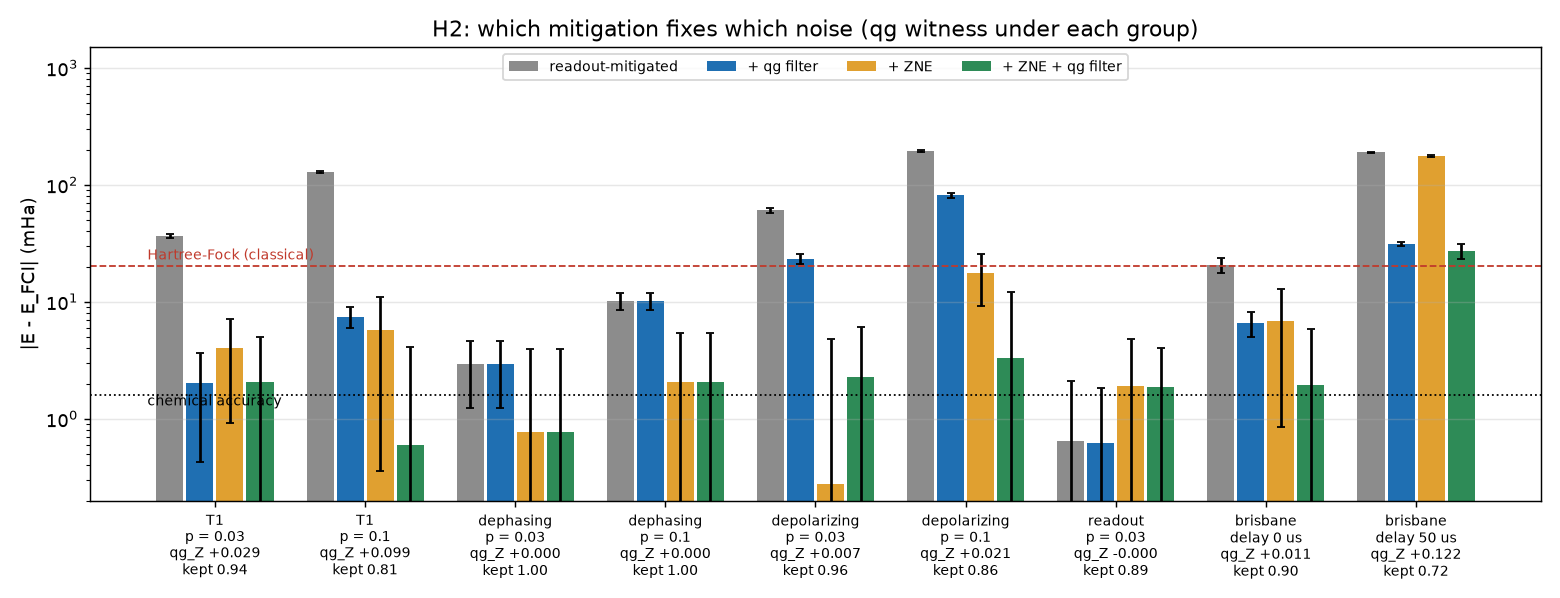
\includegraphics[width=\linewidth]{error_mitigation_qg_vs_zne.png}
\caption{Energy error of H$_2$ by noise type and mitigation (log scale). Under each group, the qg
witness and the kept fraction read from the unmitigated shots.}
\label{fig:zne}
\end{figure}

\section{Materials: 1D Hubbard dynamics}\label{sec:hubbard}

The Fermi--Hubbard chain with $L=4$ sites ($J=1$, $U=2$, 8 qubits, spin blocks in Jordan--Wigner)
evolves by first-order Trotter steps ($dt=0.25$) from a charge-density wave with sites 0 and 2
doubly occupied, a standard hardware benchmark~\cite{arute2020hubbard}. The Hamiltonian conserves
$N_\uparrow$ and $N_\downarrow$, and here \emph{every} observable of interest (charge imbalance $I$,
double occupancy $D$) is diagonal in $Z$, so the filters act on all of them. The reference is the
noiseless output of the same Trotter circuit.

On the all-to-all device (20 CX per step) the filters roughly halve the error. The spin filters add
a further 30\% at depth, as the spin leak grows from 0 to 8\%. ZNE + spin filters gives the best
double occupancy: time-averaged error 0.003 vs 0.019 raw. The witnesses stay at 0 because the noise
is unital, but the kept fraction falls from 0.88 to 0.50.

On \fb\ routing the ladder of hops and interactions costs 56 ECR per step, and routing creates spin
leak: 8, 16, 41, 45 and 47\% of the right-$N$ shots sit in the wrong spin sector after 1, 2, 4, 6 and
8 steps (H$_2$: $<1\%$). The spin filters therefore beat the $N$ filter clearly (Table~\ref{tab:hub}).
From 4 steps ($\ge188$ ECR, 18\% of shots kept) every method sits on the noise floor. $D\to1/4$,
the value of the maximally mixed state inside the spin sector, and $I\to0$ (Fig.~\ref{fig:hub}).
With the current \fb\ snapshot mostly the spin-down register drifts towards $+1$; with an older
snapshot both do. The per-register witnesses report the calibration, not a property of the method.

\begin{table}[t]
\centering\small
\caption{1D Hubbard on \fb: absolute error of $D$ and $I$ vs the noiseless Trotter circuit
(5 seeds).}
\label{tab:hub}
\begin{tabular}{lcccc}
\toprule
& $D$, 1 step & $D$, 2 steps & $I$, 1 step & $I$, 2 steps\\
\midrule
readout-mitigated & .081 & .056 & .206 & .111\\
+ $N$ filter & .050 & .029 & .124 & .070\\
+ spin filters & .039 & .016 & .100 & .047\\
+ ZNE & .031 & .031 & .036 & \textbf{.010}\\
+ ZNE + spin filters & \textbf{.009} & \textbf{.006} & \textbf{.035} & .071\\
\bottomrule
\end{tabular}
\end{table}

\begin{figure}[t]
\centering
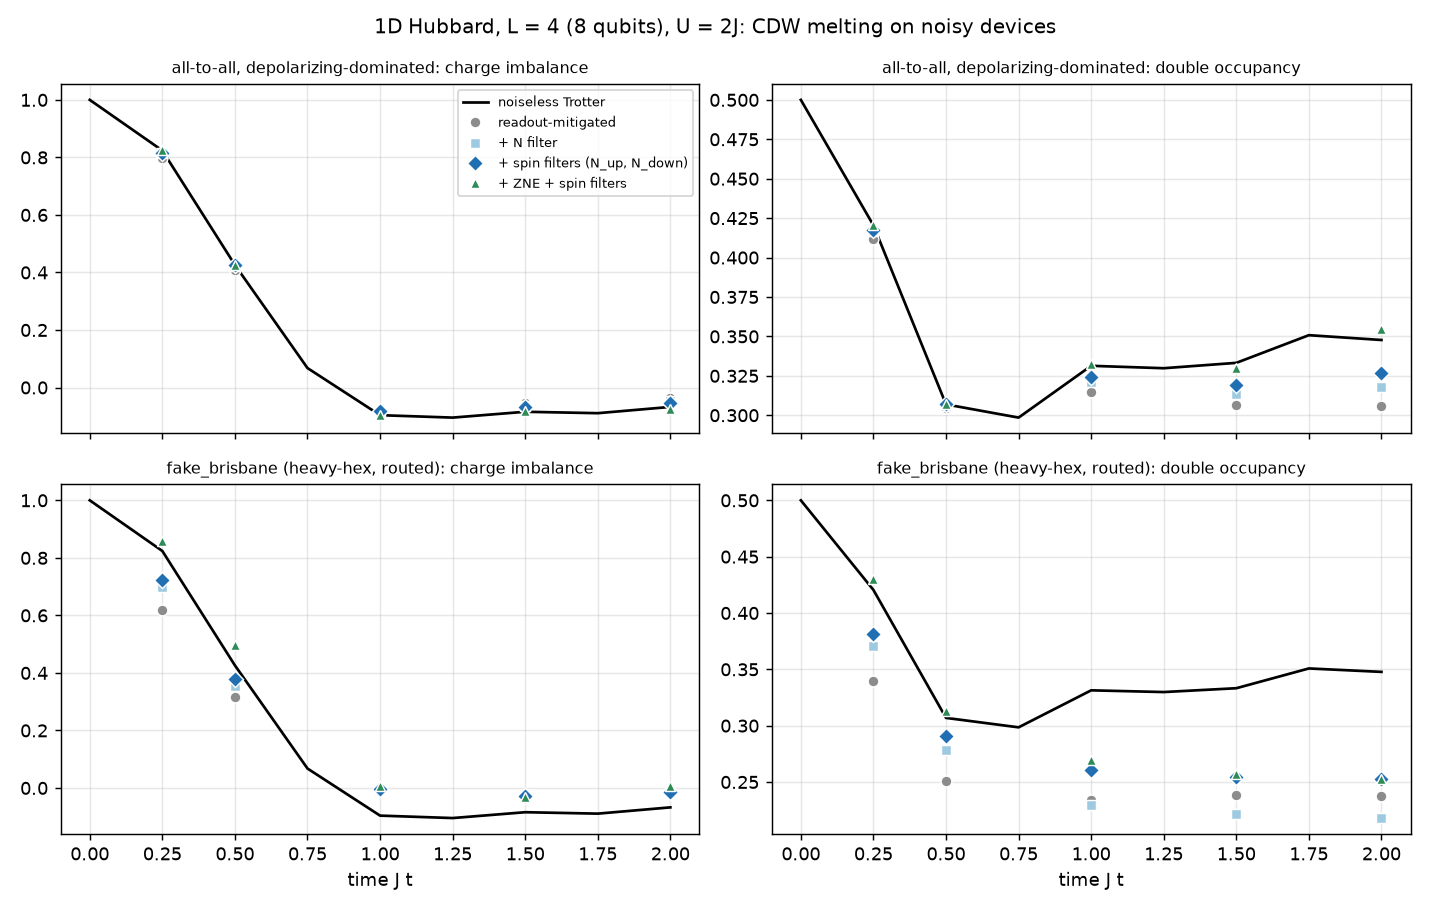
\includegraphics[width=\linewidth]{hubbard_trotter_qg_filters.png}
\caption{Charge-density-wave melting in the 1D Hubbard model on two simulated devices. Black:
noiseless Trotter circuit.}
\label{fig:hub}
\end{figure}

\section{Constrained optimization: QAOA with ``exactly \texorpdfstring{$K$}{K}''}\label{sec:qaoa}

Maximum $K$-vertex cover asks for exactly $K$ of $n$ vertices that touch the most edges. With
$x_i=(1-Z_i)/2$ the constraint is $\mqg=1-2K/n$ (0.25 for $n=8$, $K=3$). We compare standard penalty
QAOA~\cite{farhi2014}; a \emph{budget start}, with every qubit at $\qgZ=1-2K/n$ and the mixer rotated
about that axis, which needs no classical pre-solve; a warm start with
$\qgZ^{(i)}=1-2c_i$ from the LP relaxation $c$~\cite{egger2021}, clipped to $|\qgZ|\le0.5$ (Egger's
$\varepsilon=0.25$); and the constraint-preserving XY-mixer ansatz~\cite{hadfield2019} started from a
Dicke state~\cite{bartschi2019}. Angles are optimized without noise, and 4000 shots are taken on 5
random graphs $G(8,1/2)$.

On the all-to-all device (Fig.~\ref{fig:qaoa}) the filter doubles the probability that a shot is
optimal for the XY ansatz: 0.150 $\to$ 0.278 at depth 1 and 0.177 $\to$ 0.366 at depth 2. Because
that ansatz is 100\% feasible without noise, its kept fraction (0.54) is a pure error witness.
Penalty QAOA at depth $\le2$ does no better than a random feasible guess after filtering (probability
of the optimum 0.10--0.18 vs 0.096, approximation ratio 0.78 vs 0.77). The budget start raises the raw
feasibility but not the quality. The warm start is the best penalty variant, but its LP relaxation is
already integral on 3 of 5 graphs, so its value is classical. On \fb\ (134--497 ECR) every variant
ends at the random-feasible level. The kept fraction (0.24--0.33) is then close to
$\binom83/2^8=0.22$, which tells the user that no signal is left. A greedy algorithm reaches 98.5\%
of the optimum, and brute force is instant.

\begin{figure}[t]
\centering
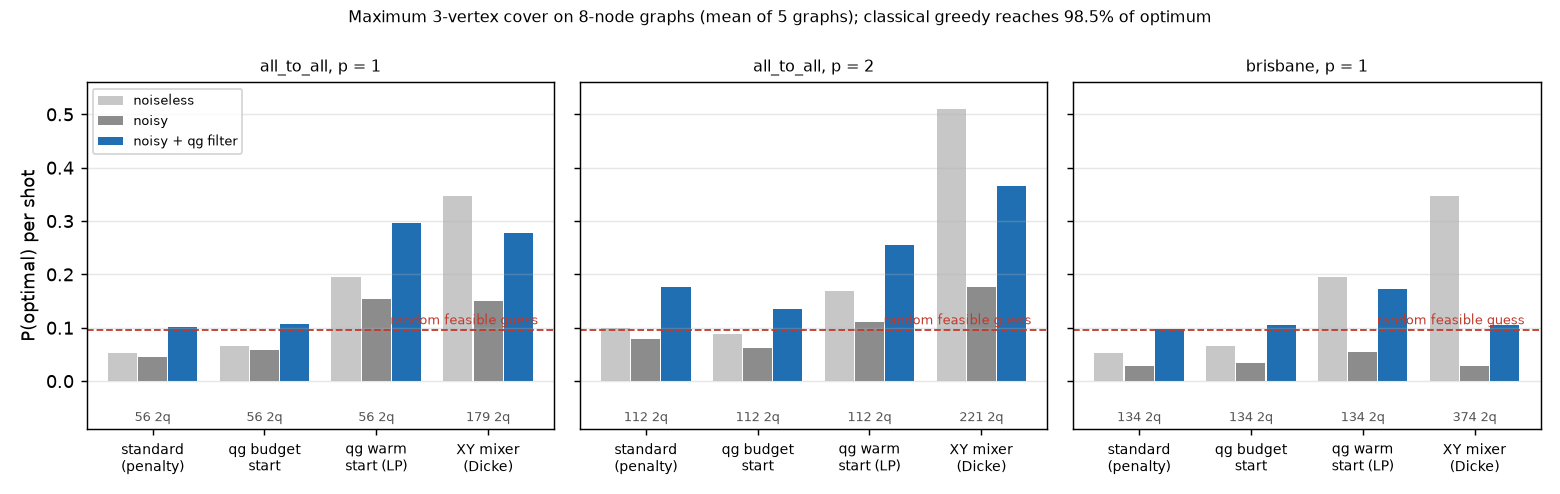
\includegraphics[width=\linewidth]{qaoa_k_constraint_qg.png}
\caption{Probability that one shot is an optimal cover, noiseless, noisy, and noisy + qg filter. The
dashed line is a random feasible guess. The number of two-qubit gates is under each group.}
\label{fig:qaoa}
\end{figure}

\section{Calibrating what the witness relies on}\label{sec:char}

Eq.~\eqref{eq:affine} makes the witness depend on $a$ and $b$. A real qubit also idles with an
excited population $p$, with $\qgZ^{\rm eq}=1-2p=\tanh(hf/2k_BT_{\rm eff})$~\cite{jin2015}. The
standard calibration prepares ``$|0\rangle$'' (the thermal state) and ``$|1\rangle$'' (X on it). From
Z-basis data alone it sees only $a+b\,\qgZ^{\rm eq}$ and $b\,\qgZ^{\rm eq}$, so it counts thermal
population as readout error.

\paragraph{Heralded sweep.} Measure once (herald), apply I, X or $R_y(\pi/2)$, wait $t$, rotate back
and measure again. For outcomes $r_1,r_2=\pm1$ at $t=0$ and a QND herald,
\begin{equation}
m=\mathbb E[r_1]=a+bq,\quad V=\mathbb E[r_1r_2\,|\,I]-m^2=b^2(1-q^2),\quad
C_X=\mathbb E[r_1r_2\,|\,X]=a^2-b^2,
\end{equation}
with $q=\qgZ^{\rm eq}$. Hence $u=bq=(m^2-V-C_X)/(2m)$, $b=\sqrt{V+u^2}$ and $a=m-u$. The delays add
$T_1$ (after X) and $T_2$ (the decay of $\qgX$ after $R_y(\pi/2)$). A joint maximum-likelihood fit of
all joint counts returns $(a,b,q,T_1,T_2)$ with the same circuit and shot budget as the standard
suite. The model is checked against a Qiskit Aer circuit that prepares the thermal state by
purification.

\paragraph{Result.} With $T_1=100~\mu$s, $T_2=70~\mu$s, $e_{01}=0.015$, $e_{10}=0.04$ and a 5~GHz
qubit (Fig.~\ref{fig:char}), the standard suite reports $T_{\rm eff}=0$ at every temperature and
overestimates $e_{01}$ by exactly $pb$ (0.0915 at $p=0.08$). The heralded sweep is unbiased: $e_{01}$
is $0.0148$--$0.0152$ and $T_{\rm eff}$ is $52.3\pm1.0$, $69.0\pm0.8$ and $98.2\pm0.9$~mK at true 52, 69
and 98~mK. Both protocols give unbiased $T_1$ and $T_2$; the joint fit is about $1.5\times$ more
precise. If the herald is not QND, with 5\% relaxation of $|1\rangle$ during it, the estimates move
by about 0.001. Separating thermal population by repeated measurement is known practice. What qg adds
is the closed form and $T_{\rm eff}$ read directly from $\qgZ^{\rm eq}$. The protocol needs
mid-circuit measurement.

\begin{figure}[t]
\centering
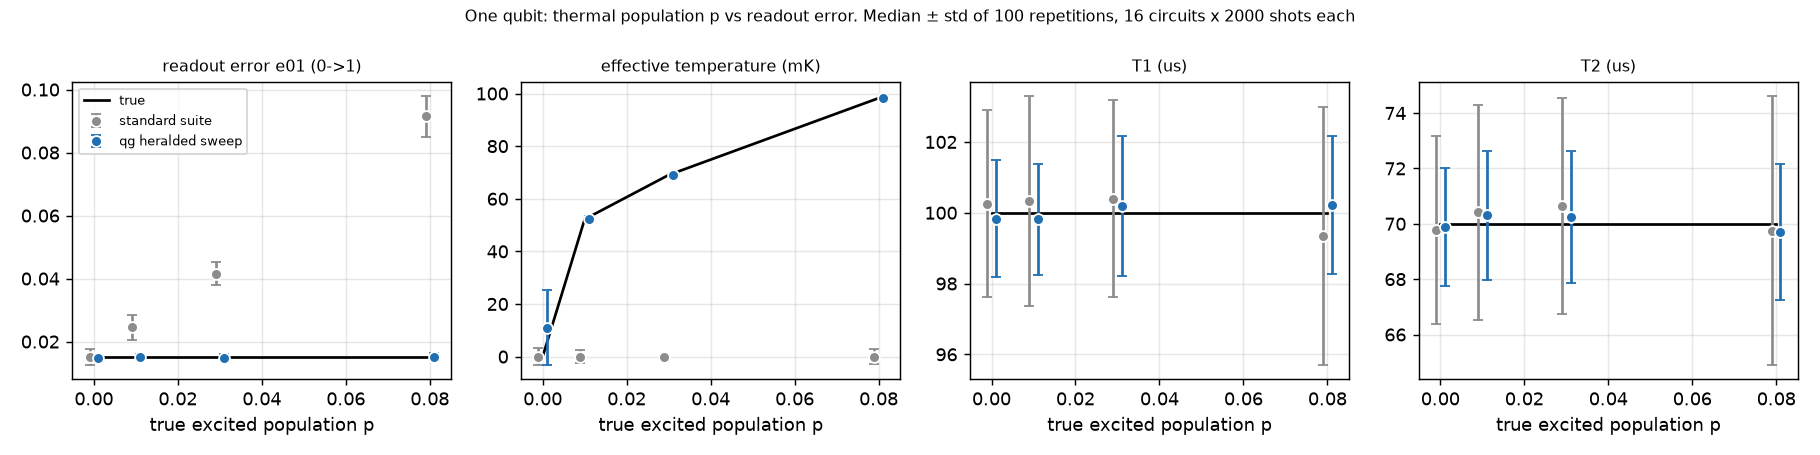
\includegraphics[width=\linewidth]{hardware_characterization_qg.png}
\caption{Standard calibration (gray) vs heralded qg sweep (blue); black: truth. Median $\pm$ std of
100 repetitions, 16 circuits $\times$ 2000 shots each.}
\label{fig:char}
\end{figure}

\section{Discussion and limitations}\label{sec:limits}

\begin{enumerate}
\item \emph{No quantum advantage.} FCI, exact diagonalization, brute force and greedy search are
exact or near-exact at every size studied. The comparisons rank strategies for a quantum
computation.
\item \emph{The filter is known}~\cite{bonetmonroig2018,mcardle2019}. The contributions are the
witness as a decision rule, the systematic comparison with ZNE and with classical baselines, and the
calibration protocol.
\item \emph{Walls.} Beyond $\sim$60 (LiH) or $\sim$190 (Hubbard, heavy-hex) noisy two-qubit gates,
unital scrambling dominates and no method helps. The witness then reports a drift towards 0 and a
kept fraction near $\binom nN/2^n$.
\item \emph{Rotated-basis terms} such as $XXYY$ cannot be filtered with Z-basis shots; they hold most
of the residual H$_2$ error.
\item \emph{Simulation only.} All devices are calibration-based or vendor noise models. Hardware runs
are prepared (IBM, IonQ) but not yet performed. The characterization protocol assumes perfect gates
and a nearly QND herald.
\item \emph{Snapshot dependence.} Per-register asymmetries depend on the calibration snapshot of the
fake backend.
\end{enumerate}

\section{Code availability}
\sloppy

All scripts, data and the regression tests that pin every number (809 tests at the time of writing)
are at \url{https://github.com/Viny2030/qang} (MIT license): \texttt{examples/chemistry\_*.py},
\texttt{error\_mitigation\_qg\_vs\_zne.py}, \texttt{hubbard\_trotter\_qg\_filters.py},
\texttt{qaoa\_k\_constraint\_qg.py}, \texttt{hardware\_characterization\_qg.py} and
\texttt{ionq\_validation.py}. Sections 20, 21, 24 and 28--31 of \texttt{RESEARCH\_NOTES.md} give
further detail.

\section*{Acknowledgments and use of AI tools}
Generative AI tools (Anthropic Claude Opus 5.5) assisted with code generation, numerical experiments,
test expansion and drafting of this text. The author framed the research questions, made the design
decisions, and reviewed, edited and validated all AI-assisted output, including every number
reported here.

\bibliographystyle{unsrtnat}
\bibliography{../refs}
\end{document}
